	\tikzset{every picture/.style={line width=0.75pt}} %set default line width to 0.75pt        
	
	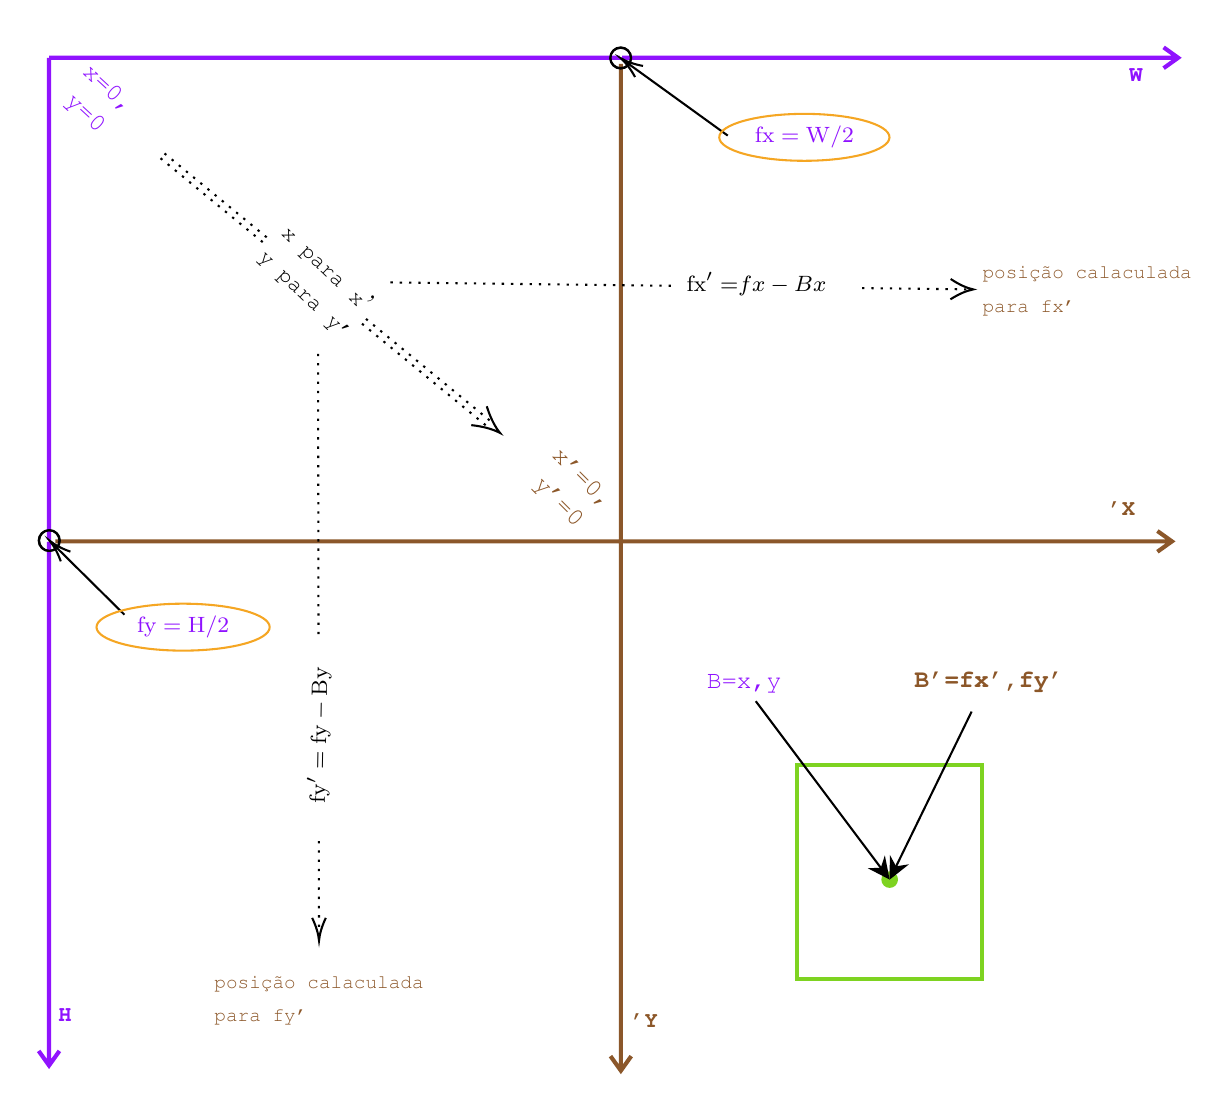
\begin{tikzpicture}[x=0.75pt,y=0.75pt,yscale=-1,xscale=1]
	%uncomment if require: \path (0,578); %set diagram left start at 0, and has height of 578
	
	%Shape: Axis 2D [id:dp745366717574464] 
	\draw [color={rgb, 255:red, 139; green, 87; blue, 42 }  ,draw opacity=1 ][line width=1.5]  (305.5,41) -- (305.5,526)(571,271) -- (33,271) (310.5,519) -- (305.5,526) -- (300.5,519) (564,266) -- (571,271) -- (564,276)  ;
	%Shape: Rectangle [id:dp835814910936395] 
	\draw  [color={rgb, 255:red, 126; green, 211; blue, 33 }  ,draw opacity=1 ][line width=1.5]  (390.5,482) -- (390.5,378.9) -- (479.5,378.9) -- (479.5,482) -- cycle ;
	%Shape: Circle [id:dp6195483350711979] 
	\draw  [color={rgb, 255:red, 126; green, 211; blue, 33 }  ,draw opacity=1 ][fill={rgb, 255:red, 126; green, 211; blue, 33 }  ,fill opacity=1 ] (431.5,433.95) .. controls (431.5,432.02) and (433.07,430.45) .. (435,430.45) .. controls (436.93,430.45) and (438.5,432.02) .. (438.5,433.95) .. controls (438.5,435.88) and (436.93,437.45) .. (435,437.45) .. controls (433.07,437.45) and (431.5,435.88) .. (431.5,433.95) -- cycle ;
	%Shape: Axis 2D [id:dp10273922885069342] 
	\draw [color={rgb, 255:red, 144; green, 19; blue, 254 }  ,draw opacity=1 ][line width=1.5]  (30,38) -- (30,523.5)(574,38) -- (30,38) -- cycle (35,516.5) -- (30,523.5) -- (25,516.5) (567,33) -- (574,38) -- (567,43)  ;
	%Straight Lines [id:da39018414566648474] 
	\draw    (370.5,348) -- (433.2,431.55) ;
	\draw [shift={(435,433.95)}, rotate = 233.11] [fill={rgb, 255:red, 0; green, 0; blue, 0 }  ][line width=0.08]  [draw opacity=0] (10.72,-5.15) -- (0,0) -- (10.72,5.15) -- (7.12,0) -- cycle    ;
	%Straight Lines [id:da811434966043961] 
	\draw    (474.5,353) -- (454.7,393.58) -- (436.32,431.25) ;
	\draw [shift={(435,433.95)}, rotate = 296.01] [fill={rgb, 255:red, 0; green, 0; blue, 0 }  ][line width=0.08]  [draw opacity=0] (10.72,-5.15) -- (0,0) -- (10.72,5.15) -- (7.12,0) -- cycle    ;
	%Straight Lines [id:da7444934143033615] 
	\draw [color={rgb, 255:red, 255; green, 255; blue, 255 }  ,draw opacity=1 ]   (306,24) -- (305.4,38.2) ;
	%Straight Lines [id:da5396729355438599] 
	\draw [color={rgb, 255:red, 255; green, 255; blue, 255 }  ,draw opacity=1 ]   (20.2,271.4) -- (30.2,270.6) ;
	%Straight Lines [id:da7044410949948923] 
	\draw    (357,75.5) -- (307.02,39.37) ;
	\draw [shift={(305.4,38.2)}, rotate = 395.86] [color={rgb, 255:red, 0; green, 0; blue, 0 }  ][line width=0.75]    (10.93,-3.29) .. controls (6.95,-1.4) and (3.31,-0.3) .. (0,0) .. controls (3.31,0.3) and (6.95,1.4) .. (10.93,3.29)   ;
	%Straight Lines [id:da8627654662164674] 
	\draw    (66.33,306.33) -- (31.62,272.01) ;
	\draw [shift={(30.2,270.6)}, rotate = 404.68] [color={rgb, 255:red, 0; green, 0; blue, 0 }  ][line width=0.75]    (10.93,-3.29) .. controls (6.95,-1.4) and (3.31,-0.3) .. (0,0) .. controls (3.31,0.3) and (6.95,1.4) .. (10.93,3.29)   ;
	
	% Text Node
	\draw (539,251) node [anchor=north west][inner sep=0.75pt]   [align=left] {{\fontfamily{pcr}\selectfont {\footnotesize \textbf{\textcolor[rgb]{0.55,0.34,0.16}{'X}}}}};
	% Text Node
	\draw (309,498) node [anchor=north west][inner sep=0.75pt]   [align=left] {{\fontfamily{pcr}\selectfont {\footnotesize \textbf{\textcolor[rgb]{0.55,0.34,0.16}{'Y}}}}};
	% Text Node
	\draw (549,42) node [anchor=north west][inner sep=0.75pt]   [align=left] {{\fontfamily{pcr}\selectfont {\footnotesize \textbf{\textcolor[rgb]{0.56,0.07,1}{W}}}}};
	% Text Node
	\draw (33,495) node [anchor=north west][inner sep=0.75pt]   [align=left] {{\fontfamily{pcr}\selectfont {\footnotesize \textbf{\textcolor[rgb]{0.56,0.07,1}{H}}}}};
	% Text Node
	\draw (364.91,339.5) node   [align=left] {{\fontfamily{pcr}\selectfont {\small \textcolor[rgb]{0.56,0.07,1}{B=x,y}}}};
	% Text Node
	\draw (31.47,39.36) node [anchor=west] [inner sep=0.75pt]  [rotate=-42.7] [align=left] {\begin{minipage}[lt]{41.469392000000006pt}\setlength\topsep{0pt}
		\begin{center}
		{\fontfamily{pcr}\selectfont {\small \textcolor[rgb]{0.56,0.07,1}{x=0, y=0}}}
		\end{center}
		
		\end{minipage}};
	% Text Node
	\draw (304.09,269.59) node [anchor=east] [inner sep=0.75pt]  [rotate=-45] [align=left] {\begin{minipage}[lt]{46.569392pt}\setlength\topsep{0pt}
		\begin{center}
		{\fontfamily{pcr}\selectfont {\small \textcolor[rgb]{0.55,0.34,0.16}{x'=0, y'=0}}}
		\end{center}
		
		\end{minipage}};
	% Text Node
	\draw (159.54,145.82) node  [rotate=-43.61] [align=left] {{\fontfamily{pcr}\selectfont {\footnotesize x para x}}'\\{\footnotesize {\fontfamily{pcr}\selectfont y para y'}}};
	% Text Node
	\draw (478.27,150.17) node [anchor=west] [inner sep=0.75pt]   [align=left] {{\fontfamily{pcr}\selectfont {\scriptsize \textcolor[rgb]{0.55,0.34,0.16}{posição calaculada}}}\\{\fontfamily{pcr}\selectfont {\scriptsize \textcolor[rgb]{0.55,0.34,0.16}{ para fx' }}}};
	% Text Node
	\draw (160.1,505.33) node [anchor=south] [inner sep=0.75pt]   [align=left] {{\fontfamily{pcr}\selectfont {\scriptsize \textcolor[rgb]{0.55,0.34,0.16}{posição calaculada}}}\\{\fontfamily{pcr}\selectfont {\scriptsize \textcolor[rgb]{0.55,0.34,0.16}{ para fy'}}}};
	% Text Node
	\draw (482.91,338.5) node   [align=left] {\textbf{{\fontfamily{pcr}\selectfont {\small \textcolor[rgb]{0.55,0.34,0.16}{B'=fx',fy'}}}}};
	% Text Node
	\draw (370.81,147) node  [font=\footnotesize]  {${\displaystyle \mathrm{fx'=} fx-Bx}$};
	% Text Node
	\draw  [color={rgb, 255:red, 245; green, 166; blue, 35 }  ,draw opacity=1 ]  (94.58, 312.33) circle [x radius= 41.72, y radius= 11.31]   ;
	\draw (94.58,312.33) node  [font=\footnotesize]  {${\displaystyle \mathrm{\textcolor[rgb]{0.56,0.07,1}{fy=H/2}}}$};
	% Text Node
	\draw  [color={rgb, 255:red, 245; green, 166; blue, 35 }  ,draw opacity=1 ]  (393.91, 76.33) circle [x radius= 41.01, y radius= 11.31]   ;
	\draw (393.91,76.33) node  [font=\footnotesize]  {${\displaystyle \mathrm{\textcolor[rgb]{0.56,0.07,1}{fx=W/2}}}$};
	% Text Node
	\draw (160.14,364.33) node  [font=\footnotesize,rotate=-271.05]  {$\mathrm{{\displaystyle fy'=fy-By}}$};
	% Connection
	\draw  [dash pattern={on 0.84pt off 2.51pt}]  (85.64,84.1) -- (136.33,125.72)(182.7,163.8) -- (242.83,213.17)(83.73,86.42) -- (134.42,128.04)(180.79,166.12) -- (240.92,215.49) ;
	\draw [shift={(247.29,218.77)}, rotate = 219.39] [color={rgb, 255:red, 0; green, 0; blue, 0 }  ][line width=0.75]    (13.12,-5.88) .. controls (8.34,-2.76) and (3.97,-0.8) .. (0,0) .. controls (3.97,0.8) and (8.34,2.76) .. (13.12,5.88)   ;
	% Connection
	\draw  [dash pattern={on 0.84pt off 2.51pt}]  (194.49,146.24) -- (329.7,147.86)(421.69,148.97) -- (473.27,149.58) ;
	\draw [shift={(475.27,149.61)}, rotate = 180.69] [color={rgb, 255:red, 0; green, 0; blue, 0 }  ][line width=0.75]    (10.93,-4.9) .. controls (6.95,-2.3) and (3.31,-0.67) .. (0,0) .. controls (3.31,0.67) and (6.95,2.3) .. (10.93,4.9)   ;
	% Connection
	\draw  [dash pattern={on 0.84pt off 2.51pt}]  (159.6,180.61) -- (159.82,316.39)(159.99,415.39) -- (160.06,461.33) ;
	\draw [shift={(160.07,463.33)}, rotate = 269.90999999999997] [color={rgb, 255:red, 0; green, 0; blue, 0 }  ][line width=0.75]    (10.93,-3.29) .. controls (6.95,-1.4) and (3.31,-0.3) .. (0,0) .. controls (3.31,0.3) and (6.95,1.4) .. (10.93,3.29)   ;
	\draw   (30, 270.62) circle [x radius= 5, y radius= 5]   ;
	\draw   (30.2, 270.6) circle [x radius= 5, y radius= 5]   ;
	\draw   (305.41, 38) circle [x radius= 5, y radius= 5]   ;
	\draw   (305.4, 38.2) circle [x radius= 5, y radius= 5]   ;
	\end{tikzpicture}
